\documentclass{article}
\usepackage[utf8]{inputenc}
\usepackage{graphicx}
\usepackage{fancyvrb} 
\usepackage{siunitx}
\usepackage[table,xcdraw, svgnames]{xcolor}
\usepackage{listings, lstautogobble}
\usepackage{subfig}

\renewcommand{\figurename}{Figuur}

\setlength{\parskip}{0.5em}

\title{Sensornetwerken top view}
\author{Groep 5}
\date{September 2018}
\pagenumbering{gobble}
\begin{document}

\maketitle
\clearpage
\pagenumbering{arabic}
\clearpage

\section*{Statemachine}
Statemachine die de verschillende states laat zien waar de Xmega in komt vanaf het opstarten.
\begin{figure}[h]
	\includegraphics[width=.8\textwidth, keepaspectratio]{media/Pstate.pdf}
    \caption{}
\end{figure}
\newpage

\section*{Message Types}
\begin{table}[h]
\begin{tabular}{|l|l|l|}
\hline
\rowcolor[HTML]{EFEFEF} 
Mask & Description           & Pipe \\ \hline
0x1  & ID Broadcast          & 0    \\ \hline
0x2  & Routine Routing Table & 1    \\ \hline
0x3  & Receive Port Data     & 1    \\ \hline
0x4  & Broadcast Reply       & 1    \\ \hline
\end{tabular}
\end{table}

\section*{Flowchart}
\begin{figure}[h]
	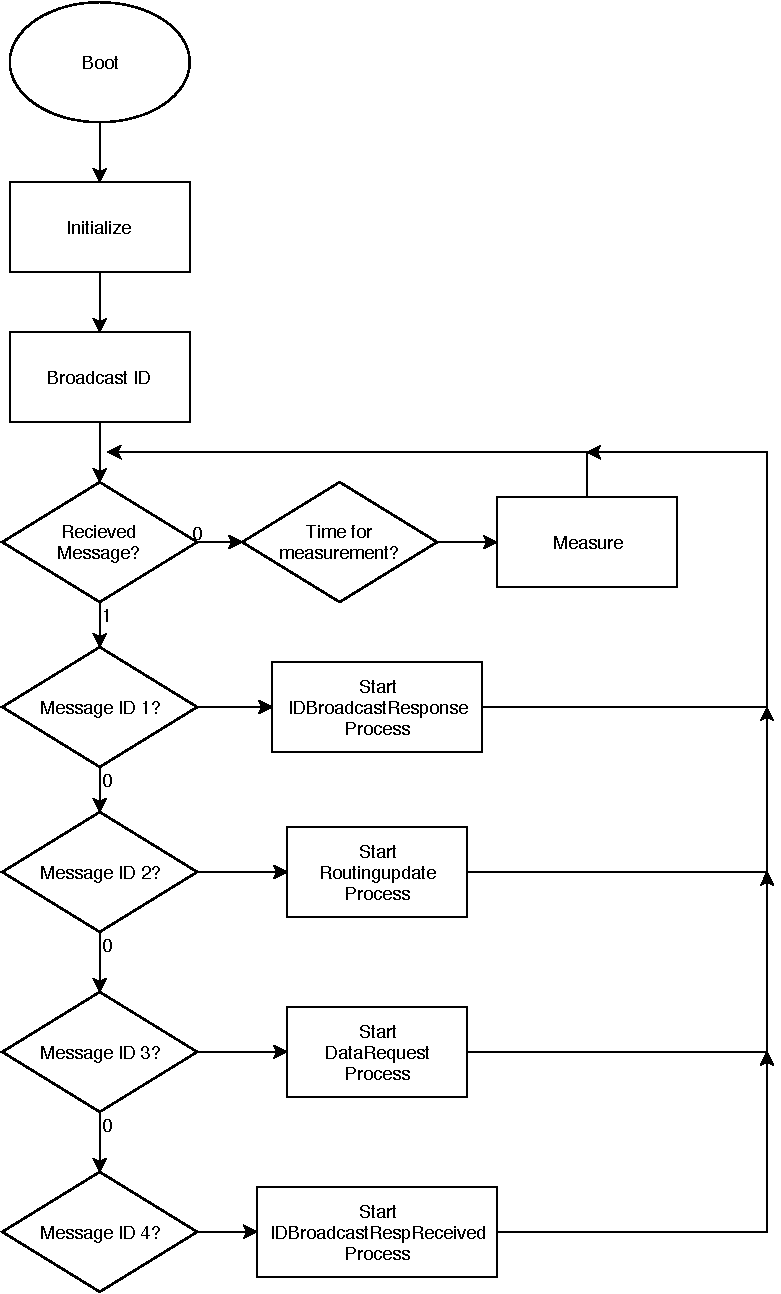
\includegraphics[width=.5\textwidth, keepaspectratio]{media/Pflow.pdf}
    \caption{}
\end{figure}

\end{document}